\documentclass[letterpaper]{article}
\usepackage[T1]{fontenc}
\usepackage{lmodern}
\pdfmapfile{+lm.map}
\usepackage[margin=0in]{geometry}
\usepackage{tikz}
\pagestyle{empty}
\renewcommand{\familydefault}{\sfdefault}
\setlength{\parindent}{0pt}
\hyphenpenalty=10000
\exhyphenpenalty=10000
\begin{document}

\null
\begin{tikzpicture}[remember picture,overlay,x=1in,y=1in]
\begin{scope}[shift={(current page.south west)}]
\node[anchor=west,inner sep=0pt,text width=7.25in,align=left,font=\fontsize{10.5}{14.5}\selectfont] at (0.62,10.5) {Week 24 / Three random decks / K--1};
\node[anchor=north west,inner sep=0pt,text width=7.2in,align=left,font=\fontsize{11.5}{15.5}\selectfont] at (0.62,10.07) {Each card has the same chance. Mix the bags separately. Draw once from each bag, then put both cards back. The bigger number wins.};
\node[anchor=north west,inner sep=0pt,text width=7.2in,align=left,font=\fontsize{16}{20}\selectfont] at (0.62,9.02) {\textbf{Problem 1:} For each of Problems 1--3, split the pairs among you and circle all nine winners on one shared page. Which deck wins more pairs?};
\node[font=\fontsize{22}{25}\selectfont] at (1.3,7.83) {A};
\draw[line width=.8pt,rounded corners=2pt] (2.12,7.3) rectangle (2.98,8.42);
\node[font=\fontsize{25}{26}\selectfont] at (2.5500000000000003,8.1512) {2};
\fill (2.41,7.67) circle (.025);
\fill (2.5500000000000003,7.67) circle (.025);
\draw[line width=.8pt,rounded corners=2pt] (3.38,7.3) rectangle (4.24,8.42);
\node[font=\fontsize{25}{26}\selectfont] at (3.81,8.1512) {4};
\fill (3.67,7.67) circle (.025);
\fill (3.81,7.67) circle (.025);
\fill (3.95,7.67) circle (.025);
\fill (3.67,7.545) circle (.025);
\draw[line width=.8pt,rounded corners=2pt] (4.640000000000001,7.3) rectangle (5.500000000000001,8.42);
\node[font=\fontsize{25}{26}\selectfont] at (5.07,8.1512) {9};
\fill (4.930000000000001,7.67) circle (.025);
\fill (5.07,7.67) circle (.025);
\fill (5.21,7.67) circle (.025);
\fill (4.930000000000001,7.545) circle (.025);
\fill (5.07,7.545) circle (.025);
\fill (5.21,7.545) circle (.025);
\fill (4.930000000000001,7.42) circle (.025);
\fill (5.07,7.42) circle (.025);
\fill (5.21,7.42) circle (.025);\node[font=\fontsize{22}{25}\selectfont] at (1.3,6.38) {B};
\draw[line width=.8pt,rounded corners=2pt] (2.12,5.85) rectangle (2.98,6.97);
\node[font=\fontsize{25}{26}\selectfont] at (2.5500000000000003,6.7012) {1};
\fill (2.41,6.22) circle (.025);
\draw[line width=.8pt,rounded corners=2pt] (3.38,5.85) rectangle (4.24,6.97);
\node[font=\fontsize{25}{26}\selectfont] at (3.81,6.7012) {6};
\fill (3.67,6.22) circle (.025);
\fill (3.81,6.22) circle (.025);
\fill (3.95,6.22) circle (.025);
\fill (3.67,6.095) circle (.025);
\fill (3.81,6.095) circle (.025);
\fill (3.95,6.095) circle (.025);
\draw[line width=.8pt,rounded corners=2pt] (4.640000000000001,5.85) rectangle (5.500000000000001,6.97);
\node[font=\fontsize{25}{26}\selectfont] at (5.07,6.7012) {8};
\fill (4.930000000000001,6.22) circle (.025);
\fill (5.07,6.22) circle (.025);
\fill (5.21,6.22) circle (.025);
\fill (4.930000000000001,6.095) circle (.025);
\fill (5.07,6.095) circle (.025);
\fill (5.21,6.095) circle (.025);
\fill (4.930000000000001,5.97) circle (.025);
\fill (5.07,5.97) circle (.025);\node[font=\fontsize{12}{15}\selectfont] at (1.405,5.02) {A};
\draw[line width=.8pt,rounded corners=2pt] (1.04,3.75) rectangle (1.77,4.85);
\node[font=\fontsize{25}{26}\selectfont] at (1.405,4.586) {2};
\fill (1.2650000000000001,4.12) circle (.025);
\fill (1.405,4.12) circle (.025);
\node[font=\fontsize{12}{15}\selectfont] at (2.4050000000000002,5.02) {B};
\draw[line width=.8pt,rounded corners=2pt] (2.04,3.75) rectangle (2.77,4.85);
\node[font=\fontsize{25}{26}\selectfont] at (2.4050000000000002,4.586) {1};
\fill (2.265,4.12) circle (.025);
\node[font=\fontsize{12}{15}\selectfont] at (3.7350000000000003,5.02) {A};
\draw[line width=.8pt,rounded corners=2pt] (3.37,3.75) rectangle (4.1,4.85);
\node[font=\fontsize{25}{26}\selectfont] at (3.7350000000000003,4.586) {2};
\fill (3.595,4.12) circle (.025);
\fill (3.7350000000000003,4.12) circle (.025);
\node[font=\fontsize{12}{15}\selectfont] at (4.735,5.02) {B};
\draw[line width=.8pt,rounded corners=2pt] (4.37,3.75) rectangle (5.1,4.85);
\node[font=\fontsize{25}{26}\selectfont] at (4.735,4.586) {6};
\fill (4.595000000000001,4.12) circle (.025);
\fill (4.735,4.12) circle (.025);
\fill (4.875,4.12) circle (.025);
\fill (4.595000000000001,3.995) circle (.025);
\fill (4.735,3.995) circle (.025);
\fill (4.875,3.995) circle (.025);
\node[font=\fontsize{12}{15}\selectfont] at (6.065,5.02) {A};
\draw[line width=.8pt,rounded corners=2pt] (5.7,3.75) rectangle (6.43,4.85);
\node[font=\fontsize{25}{26}\selectfont] at (6.065,4.586) {2};
\fill (5.925000000000001,4.12) circle (.025);
\fill (6.065,4.12) circle (.025);
\node[font=\fontsize{12}{15}\selectfont] at (7.065,5.02) {B};
\draw[line width=.8pt,rounded corners=2pt] (6.7,3.75) rectangle (7.43,4.85);
\node[font=\fontsize{25}{26}\selectfont] at (7.065,4.586) {8};
\fill (6.925000000000001,4.12) circle (.025);
\fill (7.065,4.12) circle (.025);
\fill (7.205,4.12) circle (.025);
\fill (6.925000000000001,3.995) circle (.025);
\fill (7.065,3.995) circle (.025);
\fill (7.205,3.995) circle (.025);
\fill (6.925000000000001,3.87) circle (.025);
\fill (7.065,3.87) circle (.025);
\node[font=\fontsize{12}{15}\selectfont] at (1.405,3.57) {A};
\draw[line width=.8pt,rounded corners=2pt] (1.04,2.3) rectangle (1.77,3.4);
\node[font=\fontsize{25}{26}\selectfont] at (1.405,3.136) {4};
\fill (1.2650000000000001,2.67) circle (.025);
\fill (1.405,2.67) circle (.025);
\fill (1.545,2.67) circle (.025);
\fill (1.2650000000000001,2.545) circle (.025);
\node[font=\fontsize{12}{15}\selectfont] at (2.4050000000000002,3.57) {B};
\draw[line width=.8pt,rounded corners=2pt] (2.04,2.3) rectangle (2.77,3.4);
\node[font=\fontsize{25}{26}\selectfont] at (2.4050000000000002,3.136) {1};
\fill (2.265,2.67) circle (.025);
\node[font=\fontsize{12}{15}\selectfont] at (3.7350000000000003,3.57) {A};
\draw[line width=.8pt,rounded corners=2pt] (3.37,2.3) rectangle (4.1,3.4);
\node[font=\fontsize{25}{26}\selectfont] at (3.7350000000000003,3.136) {4};
\fill (3.595,2.67) circle (.025);
\fill (3.7350000000000003,2.67) circle (.025);
\fill (3.8750000000000004,2.67) circle (.025);
\fill (3.595,2.545) circle (.025);
\node[font=\fontsize{12}{15}\selectfont] at (4.735,3.57) {B};
\draw[line width=.8pt,rounded corners=2pt] (4.37,2.3) rectangle (5.1,3.4);
\node[font=\fontsize{25}{26}\selectfont] at (4.735,3.136) {6};
\fill (4.595000000000001,2.67) circle (.025);
\fill (4.735,2.67) circle (.025);
\fill (4.875,2.67) circle (.025);
\fill (4.595000000000001,2.545) circle (.025);
\fill (4.735,2.545) circle (.025);
\fill (4.875,2.545) circle (.025);
\node[font=\fontsize{12}{15}\selectfont] at (6.065,3.57) {A};
\draw[line width=.8pt,rounded corners=2pt] (5.7,2.3) rectangle (6.43,3.4);
\node[font=\fontsize{25}{26}\selectfont] at (6.065,3.136) {4};
\fill (5.925000000000001,2.67) circle (.025);
\fill (6.065,2.67) circle (.025);
\fill (6.205,2.67) circle (.025);
\fill (5.925000000000001,2.545) circle (.025);
\node[font=\fontsize{12}{15}\selectfont] at (7.065,3.57) {B};
\draw[line width=.8pt,rounded corners=2pt] (6.7,2.3) rectangle (7.43,3.4);
\node[font=\fontsize{25}{26}\selectfont] at (7.065,3.136) {8};
\fill (6.925000000000001,2.67) circle (.025);
\fill (7.065,2.67) circle (.025);
\fill (7.205,2.67) circle (.025);
\fill (6.925000000000001,2.545) circle (.025);
\fill (7.065,2.545) circle (.025);
\fill (7.205,2.545) circle (.025);
\fill (6.925000000000001,2.42) circle (.025);
\fill (7.065,2.42) circle (.025);
\node[font=\fontsize{12}{15}\selectfont] at (1.405,2.12) {A};
\draw[line width=.8pt,rounded corners=2pt] (1.04,0.8500000000000001) rectangle (1.77,1.9500000000000002);
\node[font=\fontsize{25}{26}\selectfont] at (1.405,1.6860000000000002) {9};
\fill (1.2650000000000001,1.2200000000000002) circle (.025);
\fill (1.405,1.2200000000000002) circle (.025);
\fill (1.545,1.2200000000000002) circle (.025);
\fill (1.2650000000000001,1.0950000000000002) circle (.025);
\fill (1.405,1.0950000000000002) circle (.025);
\fill (1.545,1.0950000000000002) circle (.025);
\fill (1.2650000000000001,0.9700000000000002) circle (.025);
\fill (1.405,0.9700000000000002) circle (.025);
\fill (1.545,0.9700000000000002) circle (.025);
\node[font=\fontsize{12}{15}\selectfont] at (2.4050000000000002,2.12) {B};
\draw[line width=.8pt,rounded corners=2pt] (2.04,0.8500000000000001) rectangle (2.77,1.9500000000000002);
\node[font=\fontsize{25}{26}\selectfont] at (2.4050000000000002,1.6860000000000002) {1};
\fill (2.265,1.2200000000000002) circle (.025);
\node[font=\fontsize{12}{15}\selectfont] at (3.7350000000000003,2.12) {A};
\draw[line width=.8pt,rounded corners=2pt] (3.37,0.8500000000000001) rectangle (4.1,1.9500000000000002);
\node[font=\fontsize{25}{26}\selectfont] at (3.7350000000000003,1.6860000000000002) {9};
\fill (3.595,1.2200000000000002) circle (.025);
\fill (3.7350000000000003,1.2200000000000002) circle (.025);
\fill (3.8750000000000004,1.2200000000000002) circle (.025);
\fill (3.595,1.0950000000000002) circle (.025);
\fill (3.7350000000000003,1.0950000000000002) circle (.025);
\fill (3.8750000000000004,1.0950000000000002) circle (.025);
\fill (3.595,0.9700000000000002) circle (.025);
\fill (3.7350000000000003,0.9700000000000002) circle (.025);
\fill (3.8750000000000004,0.9700000000000002) circle (.025);
\node[font=\fontsize{12}{15}\selectfont] at (4.735,2.12) {B};
\draw[line width=.8pt,rounded corners=2pt] (4.37,0.8500000000000001) rectangle (5.1,1.9500000000000002);
\node[font=\fontsize{25}{26}\selectfont] at (4.735,1.6860000000000002) {6};
\fill (4.595000000000001,1.2200000000000002) circle (.025);
\fill (4.735,1.2200000000000002) circle (.025);
\fill (4.875,1.2200000000000002) circle (.025);
\fill (4.595000000000001,1.0950000000000002) circle (.025);
\fill (4.735,1.0950000000000002) circle (.025);
\fill (4.875,1.0950000000000002) circle (.025);
\node[font=\fontsize{12}{15}\selectfont] at (6.065,2.12) {A};
\draw[line width=.8pt,rounded corners=2pt] (5.7,0.8500000000000001) rectangle (6.43,1.9500000000000002);
\node[font=\fontsize{25}{26}\selectfont] at (6.065,1.6860000000000002) {9};
\fill (5.925000000000001,1.2200000000000002) circle (.025);
\fill (6.065,1.2200000000000002) circle (.025);
\fill (6.205,1.2200000000000002) circle (.025);
\fill (5.925000000000001,1.0950000000000002) circle (.025);
\fill (6.065,1.0950000000000002) circle (.025);
\fill (6.205,1.0950000000000002) circle (.025);
\fill (5.925000000000001,0.9700000000000002) circle (.025);
\fill (6.065,0.9700000000000002) circle (.025);
\fill (6.205,0.9700000000000002) circle (.025);
\node[font=\fontsize{12}{15}\selectfont] at (7.065,2.12) {B};
\draw[line width=.8pt,rounded corners=2pt] (6.7,0.8500000000000001) rectangle (7.43,1.9500000000000002);
\node[font=\fontsize{25}{26}\selectfont] at (7.065,1.6860000000000002) {8};
\fill (6.925000000000001,1.2200000000000002) circle (.025);
\fill (7.065,1.2200000000000002) circle (.025);
\fill (7.205,1.2200000000000002) circle (.025);
\fill (6.925000000000001,1.0950000000000002) circle (.025);
\fill (7.065,1.0950000000000002) circle (.025);
\fill (7.205,1.0950000000000002) circle (.025);
\fill (6.925000000000001,0.9700000000000002) circle (.025);
\fill (7.065,0.9700000000000002) circle (.025);
\node[anchor=west,inner sep=0pt,text width=6.7in,align=left,font=\fontsize{9.5}{13.5}\selectfont] at (0.62,0.46) {Bellingham Math Circle / Week 24 / F24-K-v2};
\node[anchor=east,inner sep=0pt,font=\fontsize{9.5}{12}\selectfont] at (7.88,.46) {1};
\end{scope}
\end{tikzpicture}
\newpage
\null
\begin{tikzpicture}[remember picture,overlay,x=1in,y=1in]
\begin{scope}[shift={(current page.south west)}]
\node[anchor=west,inner sep=0pt,text width=7.25in,align=left,font=\fontsize{10.5}{14.5}\selectfont] at (0.62,10.5) {Week 24 / Three random decks / K--1};
\node[anchor=north west,inner sep=0pt,text width=7.2in,align=left,font=\fontsize{16}{20}\selectfont] at (0.62,9.95) {\textbf{Problem 2:} Which deck wins more pairs?};
\node[font=\fontsize{22}{25}\selectfont] at (1.3,8.43) {B};
\draw[line width=.8pt,rounded corners=2pt] (2.12,7.9) rectangle (2.98,9.02);
\node[font=\fontsize{25}{26}\selectfont] at (2.5500000000000003,8.7512) {1};
\fill (2.41,8.27) circle (.025);
\draw[line width=.8pt,rounded corners=2pt] (3.38,7.9) rectangle (4.24,9.02);
\node[font=\fontsize{25}{26}\selectfont] at (3.81,8.7512) {6};
\fill (3.67,8.27) circle (.025);
\fill (3.81,8.27) circle (.025);
\fill (3.95,8.27) circle (.025);
\fill (3.67,8.145) circle (.025);
\fill (3.81,8.145) circle (.025);
\fill (3.95,8.145) circle (.025);
\draw[line width=.8pt,rounded corners=2pt] (4.640000000000001,7.9) rectangle (5.500000000000001,9.02);
\node[font=\fontsize{25}{26}\selectfont] at (5.07,8.7512) {8};
\fill (4.930000000000001,8.27) circle (.025);
\fill (5.07,8.27) circle (.025);
\fill (5.21,8.27) circle (.025);
\fill (4.930000000000001,8.145) circle (.025);
\fill (5.07,8.145) circle (.025);
\fill (5.21,8.145) circle (.025);
\fill (4.930000000000001,8.02) circle (.025);
\fill (5.07,8.02) circle (.025);\node[font=\fontsize{22}{25}\selectfont] at (1.3,6.98) {C};
\draw[line width=.8pt,rounded corners=2pt] (2.12,6.45) rectangle (2.98,7.57);
\node[font=\fontsize{25}{26}\selectfont] at (2.5500000000000003,7.301200000000001) {3};
\fill (2.41,6.82) circle (.025);
\fill (2.5500000000000003,6.82) circle (.025);
\fill (2.6900000000000004,6.82) circle (.025);
\draw[line width=.8pt,rounded corners=2pt] (3.38,6.45) rectangle (4.24,7.57);
\node[font=\fontsize{25}{26}\selectfont] at (3.81,7.301200000000001) {5};
\fill (3.67,6.82) circle (.025);
\fill (3.81,6.82) circle (.025);
\fill (3.95,6.82) circle (.025);
\fill (3.67,6.695) circle (.025);
\fill (3.81,6.695) circle (.025);
\draw[line width=.8pt,rounded corners=2pt] (4.640000000000001,6.45) rectangle (5.500000000000001,7.57);
\node[font=\fontsize{25}{26}\selectfont] at (5.07,7.301200000000001) {7};
\fill (4.930000000000001,6.82) circle (.025);
\fill (5.07,6.82) circle (.025);
\fill (5.21,6.82) circle (.025);
\fill (4.930000000000001,6.695) circle (.025);
\fill (5.07,6.695) circle (.025);
\fill (5.21,6.695) circle (.025);
\fill (4.930000000000001,6.57) circle (.025);\node[font=\fontsize{12}{15}\selectfont] at (1.405,5.02) {B};
\draw[line width=.8pt,rounded corners=2pt] (1.04,3.75) rectangle (1.77,4.85);
\node[font=\fontsize{25}{26}\selectfont] at (1.405,4.586) {1};
\fill (1.2650000000000001,4.12) circle (.025);
\node[font=\fontsize{12}{15}\selectfont] at (2.4050000000000002,5.02) {C};
\draw[line width=.8pt,rounded corners=2pt] (2.04,3.75) rectangle (2.77,4.85);
\node[font=\fontsize{25}{26}\selectfont] at (2.4050000000000002,4.586) {3};
\fill (2.265,4.12) circle (.025);
\fill (2.4050000000000002,4.12) circle (.025);
\fill (2.5450000000000004,4.12) circle (.025);
\node[font=\fontsize{12}{15}\selectfont] at (3.7350000000000003,5.02) {B};
\draw[line width=.8pt,rounded corners=2pt] (3.37,3.75) rectangle (4.1,4.85);
\node[font=\fontsize{25}{26}\selectfont] at (3.7350000000000003,4.586) {1};
\fill (3.595,4.12) circle (.025);
\node[font=\fontsize{12}{15}\selectfont] at (4.735,5.02) {C};
\draw[line width=.8pt,rounded corners=2pt] (4.37,3.75) rectangle (5.1,4.85);
\node[font=\fontsize{25}{26}\selectfont] at (4.735,4.586) {5};
\fill (4.595000000000001,4.12) circle (.025);
\fill (4.735,4.12) circle (.025);
\fill (4.875,4.12) circle (.025);
\fill (4.595000000000001,3.995) circle (.025);
\fill (4.735,3.995) circle (.025);
\node[font=\fontsize{12}{15}\selectfont] at (6.065,5.02) {B};
\draw[line width=.8pt,rounded corners=2pt] (5.7,3.75) rectangle (6.43,4.85);
\node[font=\fontsize{25}{26}\selectfont] at (6.065,4.586) {1};
\fill (5.925000000000001,4.12) circle (.025);
\node[font=\fontsize{12}{15}\selectfont] at (7.065,5.02) {C};
\draw[line width=.8pt,rounded corners=2pt] (6.7,3.75) rectangle (7.43,4.85);
\node[font=\fontsize{25}{26}\selectfont] at (7.065,4.586) {7};
\fill (6.925000000000001,4.12) circle (.025);
\fill (7.065,4.12) circle (.025);
\fill (7.205,4.12) circle (.025);
\fill (6.925000000000001,3.995) circle (.025);
\fill (7.065,3.995) circle (.025);
\fill (7.205,3.995) circle (.025);
\fill (6.925000000000001,3.87) circle (.025);
\node[font=\fontsize{12}{15}\selectfont] at (1.405,3.57) {B};
\draw[line width=.8pt,rounded corners=2pt] (1.04,2.3) rectangle (1.77,3.4);
\node[font=\fontsize{25}{26}\selectfont] at (1.405,3.136) {6};
\fill (1.2650000000000001,2.67) circle (.025);
\fill (1.405,2.67) circle (.025);
\fill (1.545,2.67) circle (.025);
\fill (1.2650000000000001,2.545) circle (.025);
\fill (1.405,2.545) circle (.025);
\fill (1.545,2.545) circle (.025);
\node[font=\fontsize{12}{15}\selectfont] at (2.4050000000000002,3.57) {C};
\draw[line width=.8pt,rounded corners=2pt] (2.04,2.3) rectangle (2.77,3.4);
\node[font=\fontsize{25}{26}\selectfont] at (2.4050000000000002,3.136) {3};
\fill (2.265,2.67) circle (.025);
\fill (2.4050000000000002,2.67) circle (.025);
\fill (2.5450000000000004,2.67) circle (.025);
\node[font=\fontsize{12}{15}\selectfont] at (3.7350000000000003,3.57) {B};
\draw[line width=.8pt,rounded corners=2pt] (3.37,2.3) rectangle (4.1,3.4);
\node[font=\fontsize{25}{26}\selectfont] at (3.7350000000000003,3.136) {6};
\fill (3.595,2.67) circle (.025);
\fill (3.7350000000000003,2.67) circle (.025);
\fill (3.8750000000000004,2.67) circle (.025);
\fill (3.595,2.545) circle (.025);
\fill (3.7350000000000003,2.545) circle (.025);
\fill (3.8750000000000004,2.545) circle (.025);
\node[font=\fontsize{12}{15}\selectfont] at (4.735,3.57) {C};
\draw[line width=.8pt,rounded corners=2pt] (4.37,2.3) rectangle (5.1,3.4);
\node[font=\fontsize{25}{26}\selectfont] at (4.735,3.136) {5};
\fill (4.595000000000001,2.67) circle (.025);
\fill (4.735,2.67) circle (.025);
\fill (4.875,2.67) circle (.025);
\fill (4.595000000000001,2.545) circle (.025);
\fill (4.735,2.545) circle (.025);
\node[font=\fontsize{12}{15}\selectfont] at (6.065,3.57) {B};
\draw[line width=.8pt,rounded corners=2pt] (5.7,2.3) rectangle (6.43,3.4);
\node[font=\fontsize{25}{26}\selectfont] at (6.065,3.136) {6};
\fill (5.925000000000001,2.67) circle (.025);
\fill (6.065,2.67) circle (.025);
\fill (6.205,2.67) circle (.025);
\fill (5.925000000000001,2.545) circle (.025);
\fill (6.065,2.545) circle (.025);
\fill (6.205,2.545) circle (.025);
\node[font=\fontsize{12}{15}\selectfont] at (7.065,3.57) {C};
\draw[line width=.8pt,rounded corners=2pt] (6.7,2.3) rectangle (7.43,3.4);
\node[font=\fontsize{25}{26}\selectfont] at (7.065,3.136) {7};
\fill (6.925000000000001,2.67) circle (.025);
\fill (7.065,2.67) circle (.025);
\fill (7.205,2.67) circle (.025);
\fill (6.925000000000001,2.545) circle (.025);
\fill (7.065,2.545) circle (.025);
\fill (7.205,2.545) circle (.025);
\fill (6.925000000000001,2.42) circle (.025);
\node[font=\fontsize{12}{15}\selectfont] at (1.405,2.12) {B};
\draw[line width=.8pt,rounded corners=2pt] (1.04,0.8500000000000001) rectangle (1.77,1.9500000000000002);
\node[font=\fontsize{25}{26}\selectfont] at (1.405,1.6860000000000002) {8};
\fill (1.2650000000000001,1.2200000000000002) circle (.025);
\fill (1.405,1.2200000000000002) circle (.025);
\fill (1.545,1.2200000000000002) circle (.025);
\fill (1.2650000000000001,1.0950000000000002) circle (.025);
\fill (1.405,1.0950000000000002) circle (.025);
\fill (1.545,1.0950000000000002) circle (.025);
\fill (1.2650000000000001,0.9700000000000002) circle (.025);
\fill (1.405,0.9700000000000002) circle (.025);
\node[font=\fontsize{12}{15}\selectfont] at (2.4050000000000002,2.12) {C};
\draw[line width=.8pt,rounded corners=2pt] (2.04,0.8500000000000001) rectangle (2.77,1.9500000000000002);
\node[font=\fontsize{25}{26}\selectfont] at (2.4050000000000002,1.6860000000000002) {3};
\fill (2.265,1.2200000000000002) circle (.025);
\fill (2.4050000000000002,1.2200000000000002) circle (.025);
\fill (2.5450000000000004,1.2200000000000002) circle (.025);
\node[font=\fontsize{12}{15}\selectfont] at (3.7350000000000003,2.12) {B};
\draw[line width=.8pt,rounded corners=2pt] (3.37,0.8500000000000001) rectangle (4.1,1.9500000000000002);
\node[font=\fontsize{25}{26}\selectfont] at (3.7350000000000003,1.6860000000000002) {8};
\fill (3.595,1.2200000000000002) circle (.025);
\fill (3.7350000000000003,1.2200000000000002) circle (.025);
\fill (3.8750000000000004,1.2200000000000002) circle (.025);
\fill (3.595,1.0950000000000002) circle (.025);
\fill (3.7350000000000003,1.0950000000000002) circle (.025);
\fill (3.8750000000000004,1.0950000000000002) circle (.025);
\fill (3.595,0.9700000000000002) circle (.025);
\fill (3.7350000000000003,0.9700000000000002) circle (.025);
\node[font=\fontsize{12}{15}\selectfont] at (4.735,2.12) {C};
\draw[line width=.8pt,rounded corners=2pt] (4.37,0.8500000000000001) rectangle (5.1,1.9500000000000002);
\node[font=\fontsize{25}{26}\selectfont] at (4.735,1.6860000000000002) {5};
\fill (4.595000000000001,1.2200000000000002) circle (.025);
\fill (4.735,1.2200000000000002) circle (.025);
\fill (4.875,1.2200000000000002) circle (.025);
\fill (4.595000000000001,1.0950000000000002) circle (.025);
\fill (4.735,1.0950000000000002) circle (.025);
\node[font=\fontsize{12}{15}\selectfont] at (6.065,2.12) {B};
\draw[line width=.8pt,rounded corners=2pt] (5.7,0.8500000000000001) rectangle (6.43,1.9500000000000002);
\node[font=\fontsize{25}{26}\selectfont] at (6.065,1.6860000000000002) {8};
\fill (5.925000000000001,1.2200000000000002) circle (.025);
\fill (6.065,1.2200000000000002) circle (.025);
\fill (6.205,1.2200000000000002) circle (.025);
\fill (5.925000000000001,1.0950000000000002) circle (.025);
\fill (6.065,1.0950000000000002) circle (.025);
\fill (6.205,1.0950000000000002) circle (.025);
\fill (5.925000000000001,0.9700000000000002) circle (.025);
\fill (6.065,0.9700000000000002) circle (.025);
\node[font=\fontsize{12}{15}\selectfont] at (7.065,2.12) {C};
\draw[line width=.8pt,rounded corners=2pt] (6.7,0.8500000000000001) rectangle (7.43,1.9500000000000002);
\node[font=\fontsize{25}{26}\selectfont] at (7.065,1.6860000000000002) {7};
\fill (6.925000000000001,1.2200000000000002) circle (.025);
\fill (7.065,1.2200000000000002) circle (.025);
\fill (7.205,1.2200000000000002) circle (.025);
\fill (6.925000000000001,1.0950000000000002) circle (.025);
\fill (7.065,1.0950000000000002) circle (.025);
\fill (7.205,1.0950000000000002) circle (.025);
\fill (6.925000000000001,0.9700000000000002) circle (.025);
\node[anchor=west,inner sep=0pt,text width=6.7in,align=left,font=\fontsize{9.5}{13.5}\selectfont] at (0.62,0.46) {Bellingham Math Circle / Week 24 / F24-K-v2};
\node[anchor=east,inner sep=0pt,font=\fontsize{9.5}{12}\selectfont] at (7.88,.46) {2};
\end{scope}
\end{tikzpicture}
\newpage
\null
\begin{tikzpicture}[remember picture,overlay,x=1in,y=1in]
\begin{scope}[shift={(current page.south west)}]
\node[anchor=west,inner sep=0pt,text width=7.25in,align=left,font=\fontsize{10.5}{14.5}\selectfont] at (0.62,10.5) {Week 24 / Three random decks / K--1};
\node[anchor=north west,inner sep=0pt,text width=7.2in,align=left,font=\fontsize{16}{20}\selectfont] at (0.62,9.95) {\textbf{Problem 3:} Does any of A, B, and C win more pairs than both other decks?};
\node[font=\fontsize{22}{25}\selectfont] at (1.3,8.43) {C};
\draw[line width=.8pt,rounded corners=2pt] (2.12,7.9) rectangle (2.98,9.02);
\node[font=\fontsize{25}{26}\selectfont] at (2.5500000000000003,8.7512) {3};
\fill (2.41,8.27) circle (.025);
\fill (2.5500000000000003,8.27) circle (.025);
\fill (2.6900000000000004,8.27) circle (.025);
\draw[line width=.8pt,rounded corners=2pt] (3.38,7.9) rectangle (4.24,9.02);
\node[font=\fontsize{25}{26}\selectfont] at (3.81,8.7512) {5};
\fill (3.67,8.27) circle (.025);
\fill (3.81,8.27) circle (.025);
\fill (3.95,8.27) circle (.025);
\fill (3.67,8.145) circle (.025);
\fill (3.81,8.145) circle (.025);
\draw[line width=.8pt,rounded corners=2pt] (4.640000000000001,7.9) rectangle (5.500000000000001,9.02);
\node[font=\fontsize{25}{26}\selectfont] at (5.07,8.7512) {7};
\fill (4.930000000000001,8.27) circle (.025);
\fill (5.07,8.27) circle (.025);
\fill (5.21,8.27) circle (.025);
\fill (4.930000000000001,8.145) circle (.025);
\fill (5.07,8.145) circle (.025);
\fill (5.21,8.145) circle (.025);
\fill (4.930000000000001,8.02) circle (.025);\node[font=\fontsize{22}{25}\selectfont] at (1.3,6.98) {A};
\draw[line width=.8pt,rounded corners=2pt] (2.12,6.45) rectangle (2.98,7.57);
\node[font=\fontsize{25}{26}\selectfont] at (2.5500000000000003,7.301200000000001) {2};
\fill (2.41,6.82) circle (.025);
\fill (2.5500000000000003,6.82) circle (.025);
\draw[line width=.8pt,rounded corners=2pt] (3.38,6.45) rectangle (4.24,7.57);
\node[font=\fontsize{25}{26}\selectfont] at (3.81,7.301200000000001) {4};
\fill (3.67,6.82) circle (.025);
\fill (3.81,6.82) circle (.025);
\fill (3.95,6.82) circle (.025);
\fill (3.67,6.695) circle (.025);
\draw[line width=.8pt,rounded corners=2pt] (4.640000000000001,6.45) rectangle (5.500000000000001,7.57);
\node[font=\fontsize{25}{26}\selectfont] at (5.07,7.301200000000001) {9};
\fill (4.930000000000001,6.82) circle (.025);
\fill (5.07,6.82) circle (.025);
\fill (5.21,6.82) circle (.025);
\fill (4.930000000000001,6.695) circle (.025);
\fill (5.07,6.695) circle (.025);
\fill (5.21,6.695) circle (.025);
\fill (4.930000000000001,6.57) circle (.025);
\fill (5.07,6.57) circle (.025);
\fill (5.21,6.57) circle (.025);\node[font=\fontsize{12}{15}\selectfont] at (1.405,5.02) {C};
\draw[line width=.8pt,rounded corners=2pt] (1.04,3.75) rectangle (1.77,4.85);
\node[font=\fontsize{25}{26}\selectfont] at (1.405,4.586) {3};
\fill (1.2650000000000001,4.12) circle (.025);
\fill (1.405,4.12) circle (.025);
\fill (1.545,4.12) circle (.025);
\node[font=\fontsize{12}{15}\selectfont] at (2.4050000000000002,5.02) {A};
\draw[line width=.8pt,rounded corners=2pt] (2.04,3.75) rectangle (2.77,4.85);
\node[font=\fontsize{25}{26}\selectfont] at (2.4050000000000002,4.586) {2};
\fill (2.265,4.12) circle (.025);
\fill (2.4050000000000002,4.12) circle (.025);
\node[font=\fontsize{12}{15}\selectfont] at (3.7350000000000003,5.02) {C};
\draw[line width=.8pt,rounded corners=2pt] (3.37,3.75) rectangle (4.1,4.85);
\node[font=\fontsize{25}{26}\selectfont] at (3.7350000000000003,4.586) {3};
\fill (3.595,4.12) circle (.025);
\fill (3.7350000000000003,4.12) circle (.025);
\fill (3.8750000000000004,4.12) circle (.025);
\node[font=\fontsize{12}{15}\selectfont] at (4.735,5.02) {A};
\draw[line width=.8pt,rounded corners=2pt] (4.37,3.75) rectangle (5.1,4.85);
\node[font=\fontsize{25}{26}\selectfont] at (4.735,4.586) {4};
\fill (4.595000000000001,4.12) circle (.025);
\fill (4.735,4.12) circle (.025);
\fill (4.875,4.12) circle (.025);
\fill (4.595000000000001,3.995) circle (.025);
\node[font=\fontsize{12}{15}\selectfont] at (6.065,5.02) {C};
\draw[line width=.8pt,rounded corners=2pt] (5.7,3.75) rectangle (6.43,4.85);
\node[font=\fontsize{25}{26}\selectfont] at (6.065,4.586) {3};
\fill (5.925000000000001,4.12) circle (.025);
\fill (6.065,4.12) circle (.025);
\fill (6.205,4.12) circle (.025);
\node[font=\fontsize{12}{15}\selectfont] at (7.065,5.02) {A};
\draw[line width=.8pt,rounded corners=2pt] (6.7,3.75) rectangle (7.43,4.85);
\node[font=\fontsize{25}{26}\selectfont] at (7.065,4.586) {9};
\fill (6.925000000000001,4.12) circle (.025);
\fill (7.065,4.12) circle (.025);
\fill (7.205,4.12) circle (.025);
\fill (6.925000000000001,3.995) circle (.025);
\fill (7.065,3.995) circle (.025);
\fill (7.205,3.995) circle (.025);
\fill (6.925000000000001,3.87) circle (.025);
\fill (7.065,3.87) circle (.025);
\fill (7.205,3.87) circle (.025);
\node[font=\fontsize{12}{15}\selectfont] at (1.405,3.57) {C};
\draw[line width=.8pt,rounded corners=2pt] (1.04,2.3) rectangle (1.77,3.4);
\node[font=\fontsize{25}{26}\selectfont] at (1.405,3.136) {5};
\fill (1.2650000000000001,2.67) circle (.025);
\fill (1.405,2.67) circle (.025);
\fill (1.545,2.67) circle (.025);
\fill (1.2650000000000001,2.545) circle (.025);
\fill (1.405,2.545) circle (.025);
\node[font=\fontsize{12}{15}\selectfont] at (2.4050000000000002,3.57) {A};
\draw[line width=.8pt,rounded corners=2pt] (2.04,2.3) rectangle (2.77,3.4);
\node[font=\fontsize{25}{26}\selectfont] at (2.4050000000000002,3.136) {2};
\fill (2.265,2.67) circle (.025);
\fill (2.4050000000000002,2.67) circle (.025);
\node[font=\fontsize{12}{15}\selectfont] at (3.7350000000000003,3.57) {C};
\draw[line width=.8pt,rounded corners=2pt] (3.37,2.3) rectangle (4.1,3.4);
\node[font=\fontsize{25}{26}\selectfont] at (3.7350000000000003,3.136) {5};
\fill (3.595,2.67) circle (.025);
\fill (3.7350000000000003,2.67) circle (.025);
\fill (3.8750000000000004,2.67) circle (.025);
\fill (3.595,2.545) circle (.025);
\fill (3.7350000000000003,2.545) circle (.025);
\node[font=\fontsize{12}{15}\selectfont] at (4.735,3.57) {A};
\draw[line width=.8pt,rounded corners=2pt] (4.37,2.3) rectangle (5.1,3.4);
\node[font=\fontsize{25}{26}\selectfont] at (4.735,3.136) {4};
\fill (4.595000000000001,2.67) circle (.025);
\fill (4.735,2.67) circle (.025);
\fill (4.875,2.67) circle (.025);
\fill (4.595000000000001,2.545) circle (.025);
\node[font=\fontsize{12}{15}\selectfont] at (6.065,3.57) {C};
\draw[line width=.8pt,rounded corners=2pt] (5.7,2.3) rectangle (6.43,3.4);
\node[font=\fontsize{25}{26}\selectfont] at (6.065,3.136) {5};
\fill (5.925000000000001,2.67) circle (.025);
\fill (6.065,2.67) circle (.025);
\fill (6.205,2.67) circle (.025);
\fill (5.925000000000001,2.545) circle (.025);
\fill (6.065,2.545) circle (.025);
\node[font=\fontsize{12}{15}\selectfont] at (7.065,3.57) {A};
\draw[line width=.8pt,rounded corners=2pt] (6.7,2.3) rectangle (7.43,3.4);
\node[font=\fontsize{25}{26}\selectfont] at (7.065,3.136) {9};
\fill (6.925000000000001,2.67) circle (.025);
\fill (7.065,2.67) circle (.025);
\fill (7.205,2.67) circle (.025);
\fill (6.925000000000001,2.545) circle (.025);
\fill (7.065,2.545) circle (.025);
\fill (7.205,2.545) circle (.025);
\fill (6.925000000000001,2.42) circle (.025);
\fill (7.065,2.42) circle (.025);
\fill (7.205,2.42) circle (.025);
\node[font=\fontsize{12}{15}\selectfont] at (1.405,2.12) {C};
\draw[line width=.8pt,rounded corners=2pt] (1.04,0.8500000000000001) rectangle (1.77,1.9500000000000002);
\node[font=\fontsize{25}{26}\selectfont] at (1.405,1.6860000000000002) {7};
\fill (1.2650000000000001,1.2200000000000002) circle (.025);
\fill (1.405,1.2200000000000002) circle (.025);
\fill (1.545,1.2200000000000002) circle (.025);
\fill (1.2650000000000001,1.0950000000000002) circle (.025);
\fill (1.405,1.0950000000000002) circle (.025);
\fill (1.545,1.0950000000000002) circle (.025);
\fill (1.2650000000000001,0.9700000000000002) circle (.025);
\node[font=\fontsize{12}{15}\selectfont] at (2.4050000000000002,2.12) {A};
\draw[line width=.8pt,rounded corners=2pt] (2.04,0.8500000000000001) rectangle (2.77,1.9500000000000002);
\node[font=\fontsize{25}{26}\selectfont] at (2.4050000000000002,1.6860000000000002) {2};
\fill (2.265,1.2200000000000002) circle (.025);
\fill (2.4050000000000002,1.2200000000000002) circle (.025);
\node[font=\fontsize{12}{15}\selectfont] at (3.7350000000000003,2.12) {C};
\draw[line width=.8pt,rounded corners=2pt] (3.37,0.8500000000000001) rectangle (4.1,1.9500000000000002);
\node[font=\fontsize{25}{26}\selectfont] at (3.7350000000000003,1.6860000000000002) {7};
\fill (3.595,1.2200000000000002) circle (.025);
\fill (3.7350000000000003,1.2200000000000002) circle (.025);
\fill (3.8750000000000004,1.2200000000000002) circle (.025);
\fill (3.595,1.0950000000000002) circle (.025);
\fill (3.7350000000000003,1.0950000000000002) circle (.025);
\fill (3.8750000000000004,1.0950000000000002) circle (.025);
\fill (3.595,0.9700000000000002) circle (.025);
\node[font=\fontsize{12}{15}\selectfont] at (4.735,2.12) {A};
\draw[line width=.8pt,rounded corners=2pt] (4.37,0.8500000000000001) rectangle (5.1,1.9500000000000002);
\node[font=\fontsize{25}{26}\selectfont] at (4.735,1.6860000000000002) {4};
\fill (4.595000000000001,1.2200000000000002) circle (.025);
\fill (4.735,1.2200000000000002) circle (.025);
\fill (4.875,1.2200000000000002) circle (.025);
\fill (4.595000000000001,1.0950000000000002) circle (.025);
\node[font=\fontsize{12}{15}\selectfont] at (6.065,2.12) {C};
\draw[line width=.8pt,rounded corners=2pt] (5.7,0.8500000000000001) rectangle (6.43,1.9500000000000002);
\node[font=\fontsize{25}{26}\selectfont] at (6.065,1.6860000000000002) {7};
\fill (5.925000000000001,1.2200000000000002) circle (.025);
\fill (6.065,1.2200000000000002) circle (.025);
\fill (6.205,1.2200000000000002) circle (.025);
\fill (5.925000000000001,1.0950000000000002) circle (.025);
\fill (6.065,1.0950000000000002) circle (.025);
\fill (6.205,1.0950000000000002) circle (.025);
\fill (5.925000000000001,0.9700000000000002) circle (.025);
\node[font=\fontsize{12}{15}\selectfont] at (7.065,2.12) {A};
\draw[line width=.8pt,rounded corners=2pt] (6.7,0.8500000000000001) rectangle (7.43,1.9500000000000002);
\node[font=\fontsize{25}{26}\selectfont] at (7.065,1.6860000000000002) {9};
\fill (6.925000000000001,1.2200000000000002) circle (.025);
\fill (7.065,1.2200000000000002) circle (.025);
\fill (7.205,1.2200000000000002) circle (.025);
\fill (6.925000000000001,1.0950000000000002) circle (.025);
\fill (7.065,1.0950000000000002) circle (.025);
\fill (7.205,1.0950000000000002) circle (.025);
\fill (6.925000000000001,0.9700000000000002) circle (.025);
\fill (7.065,0.9700000000000002) circle (.025);
\fill (7.205,0.9700000000000002) circle (.025);
\node[anchor=west,inner sep=0pt,text width=6.7in,align=left,font=\fontsize{9.5}{13.5}\selectfont] at (0.62,0.46) {Bellingham Math Circle / Week 24 / F24-K-v2};
\node[anchor=east,inner sep=0pt,font=\fontsize{9.5}{12}\selectfont] at (7.88,.46) {3};
\end{scope}
\end{tikzpicture}
\newpage
\null
\begin{tikzpicture}[remember picture,overlay,x=1in,y=1in]
\begin{scope}[shift={(current page.south west)}]
\node[anchor=west,inner sep=0pt,text width=7.25in,align=left,font=\fontsize{10.5}{14.5}\selectfont] at (0.62,10.5) {Week 24 / Three random decks / K--1};
\node[anchor=north west,inner sep=0pt,text width=7.2in,align=left,font=\fontsize{16}{20}\selectfont] at (0.62,9.95) {\textbf{Problem 4:} For each of A, B, and C, choose a deck that wins more card pairs and play six rounds. Must your chosen deck win more rounds?};
\node[font=\fontsize{22}{25}\selectfont] at (1.3,8.43) {A};
\draw[line width=.8pt,rounded corners=2pt] (2.12,7.9) rectangle (2.98,9.02);
\node[font=\fontsize{25}{26}\selectfont] at (2.5500000000000003,8.7512) {2};
\fill (2.41,8.27) circle (.025);
\fill (2.5500000000000003,8.27) circle (.025);
\draw[line width=.8pt,rounded corners=2pt] (3.38,7.9) rectangle (4.24,9.02);
\node[font=\fontsize{25}{26}\selectfont] at (3.81,8.7512) {4};
\fill (3.67,8.27) circle (.025);
\fill (3.81,8.27) circle (.025);
\fill (3.95,8.27) circle (.025);
\fill (3.67,8.145) circle (.025);
\draw[line width=.8pt,rounded corners=2pt] (4.640000000000001,7.9) rectangle (5.500000000000001,9.02);
\node[font=\fontsize{25}{26}\selectfont] at (5.07,8.7512) {9};
\fill (4.930000000000001,8.27) circle (.025);
\fill (5.07,8.27) circle (.025);
\fill (5.21,8.27) circle (.025);
\fill (4.930000000000001,8.145) circle (.025);
\fill (5.07,8.145) circle (.025);
\fill (5.21,8.145) circle (.025);
\fill (4.930000000000001,8.02) circle (.025);
\fill (5.07,8.02) circle (.025);
\fill (5.21,8.02) circle (.025);\node[font=\fontsize{22}{25}\selectfont] at (1.3,7.03) {B};
\draw[line width=.8pt,rounded corners=2pt] (2.12,6.5) rectangle (2.98,7.62);
\node[font=\fontsize{25}{26}\selectfont] at (2.5500000000000003,7.3512) {1};
\fill (2.41,6.87) circle (.025);
\draw[line width=.8pt,rounded corners=2pt] (3.38,6.5) rectangle (4.24,7.62);
\node[font=\fontsize{25}{26}\selectfont] at (3.81,7.3512) {6};
\fill (3.67,6.87) circle (.025);
\fill (3.81,6.87) circle (.025);
\fill (3.95,6.87) circle (.025);
\fill (3.67,6.745) circle (.025);
\fill (3.81,6.745) circle (.025);
\fill (3.95,6.745) circle (.025);
\draw[line width=.8pt,rounded corners=2pt] (4.640000000000001,6.5) rectangle (5.500000000000001,7.62);
\node[font=\fontsize{25}{26}\selectfont] at (5.07,7.3512) {8};
\fill (4.930000000000001,6.87) circle (.025);
\fill (5.07,6.87) circle (.025);
\fill (5.21,6.87) circle (.025);
\fill (4.930000000000001,6.745) circle (.025);
\fill (5.07,6.745) circle (.025);
\fill (5.21,6.745) circle (.025);
\fill (4.930000000000001,6.62) circle (.025);
\fill (5.07,6.62) circle (.025);\node[font=\fontsize{22}{25}\selectfont] at (1.3,5.63) {C};
\draw[line width=.8pt,rounded corners=2pt] (2.12,5.1) rectangle (2.98,6.22);
\node[font=\fontsize{25}{26}\selectfont] at (2.5500000000000003,5.9512) {3};
\fill (2.41,5.47) circle (.025);
\fill (2.5500000000000003,5.47) circle (.025);
\fill (2.6900000000000004,5.47) circle (.025);
\draw[line width=.8pt,rounded corners=2pt] (3.38,5.1) rectangle (4.24,6.22);
\node[font=\fontsize{25}{26}\selectfont] at (3.81,5.9512) {5};
\fill (3.67,5.47) circle (.025);
\fill (3.81,5.47) circle (.025);
\fill (3.95,5.47) circle (.025);
\fill (3.67,5.345) circle (.025);
\fill (3.81,5.345) circle (.025);
\draw[line width=.8pt,rounded corners=2pt] (4.640000000000001,5.1) rectangle (5.500000000000001,6.22);
\node[font=\fontsize{25}{26}\selectfont] at (5.07,5.9512) {7};
\fill (4.930000000000001,5.47) circle (.025);
\fill (5.07,5.47) circle (.025);
\fill (5.21,5.47) circle (.025);
\fill (4.930000000000001,5.345) circle (.025);
\fill (5.07,5.345) circle (.025);
\fill (5.21,5.345) circle (.025);
\fill (4.930000000000001,5.22) circle (.025);
\node[anchor=west,inner sep=0pt,text width=6.7in,align=left,font=\fontsize{9.5}{13.5}\selectfont] at (0.62,0.46) {Bellingham Math Circle / Week 24 / F24-K-v2};
\node[anchor=east,inner sep=0pt,font=\fontsize{9.5}{12}\selectfont] at (7.88,.46) {4};
\end{scope}
\end{tikzpicture}
\newpage
\null
\begin{tikzpicture}[remember picture,overlay,x=1in,y=1in]
\begin{scope}[shift={(current page.south west)}]
\node[anchor=west,inner sep=0pt,text width=7.25in,align=left,font=\fontsize{10.5}{14.5}\selectfont] at (0.62,10.5) {Week 24 / Three random decks / K--1};
\node[anchor=north west,inner sep=0pt,text width=7.2in,align=left,font=\fontsize{16}{20}\selectfont] at (0.62,9.95) {\textbf{Problem 5:} Try 3, 5, 7, and 9 in A's empty place. Which choices make A win more card pairs than B?};
\node[font=\fontsize{22}{25}\selectfont] at (1.3,8.33) {A};
\draw[line width=.8pt,rounded corners=2pt] (2.12,7.8) rectangle (2.98,8.92);
\node[font=\fontsize{25}{26}\selectfont] at (2.5500000000000003,8.6512) {2};
\fill (2.41,8.17) circle (.025);
\fill (2.5500000000000003,8.17) circle (.025);
\draw[line width=.8pt,rounded corners=2pt] (3.38,7.8) rectangle (4.24,8.92);
\node[font=\fontsize{25}{26}\selectfont] at (3.81,8.6512) {4};
\fill (3.67,8.17) circle (.025);
\fill (3.81,8.17) circle (.025);
\fill (3.95,8.17) circle (.025);
\fill (3.67,8.045) circle (.025);
\draw[line width=.8pt,rounded corners=2pt] (4.640000000000001,7.8) rectangle (5.500000000000001,8.92);\node[font=\fontsize{22}{25}\selectfont] at (1.3,6.930000000000001) {B};
\draw[line width=.8pt,rounded corners=2pt] (2.12,6.4) rectangle (2.98,7.5200000000000005);
\node[font=\fontsize{25}{26}\selectfont] at (2.5500000000000003,7.251200000000001) {1};
\fill (2.41,6.7700000000000005) circle (.025);
\draw[line width=.8pt,rounded corners=2pt] (3.38,6.4) rectangle (4.24,7.5200000000000005);
\node[font=\fontsize{25}{26}\selectfont] at (3.81,7.251200000000001) {6};
\fill (3.67,6.7700000000000005) circle (.025);
\fill (3.81,6.7700000000000005) circle (.025);
\fill (3.95,6.7700000000000005) circle (.025);
\fill (3.67,6.6450000000000005) circle (.025);
\fill (3.81,6.6450000000000005) circle (.025);
\fill (3.95,6.6450000000000005) circle (.025);
\draw[line width=.8pt,rounded corners=2pt] (4.640000000000001,6.4) rectangle (5.500000000000001,7.5200000000000005);
\node[font=\fontsize{25}{26}\selectfont] at (5.07,7.251200000000001) {8};
\fill (4.930000000000001,6.7700000000000005) circle (.025);
\fill (5.07,6.7700000000000005) circle (.025);
\fill (5.21,6.7700000000000005) circle (.025);
\fill (4.930000000000001,6.6450000000000005) circle (.025);
\fill (5.07,6.6450000000000005) circle (.025);
\fill (5.21,6.6450000000000005) circle (.025);
\fill (4.930000000000001,6.5200000000000005) circle (.025);
\fill (5.07,6.5200000000000005) circle (.025);\draw[line width=.8pt,rounded corners=2pt] (2.355,4.85) rectangle (3.085,5.949999999999999);
\node[font=\fontsize{25}{26}\selectfont] at (2.7199999999999998,5.686) {3};
\fill (2.5799999999999996,5.22) circle (.025);
\fill (2.7199999999999998,5.22) circle (.025);
\fill (2.86,5.22) circle (.025);
\draw[line width=.8pt,rounded corners=2pt] (3.375,4.85) rectangle (4.105,5.949999999999999);
\node[font=\fontsize{25}{26}\selectfont] at (3.74,5.686) {5};
\fill (3.6,5.22) circle (.025);
\fill (3.74,5.22) circle (.025);
\fill (3.8800000000000003,5.22) circle (.025);
\fill (3.6,5.095) circle (.025);
\fill (3.74,5.095) circle (.025);
\draw[line width=.8pt,rounded corners=2pt] (4.395,4.85) rectangle (5.125,5.949999999999999);
\node[font=\fontsize{25}{26}\selectfont] at (4.76,5.686) {7};
\fill (4.62,5.22) circle (.025);
\fill (4.76,5.22) circle (.025);
\fill (4.8999999999999995,5.22) circle (.025);
\fill (4.62,5.095) circle (.025);
\fill (4.76,5.095) circle (.025);
\fill (4.8999999999999995,5.095) circle (.025);
\fill (4.62,4.97) circle (.025);
\draw[line width=.8pt,rounded corners=2pt] (5.415,4.85) rectangle (6.145,5.949999999999999);
\node[font=\fontsize{25}{26}\selectfont] at (5.78,5.686) {9};
\fill (5.640000000000001,5.22) circle (.025);
\fill (5.78,5.22) circle (.025);
\fill (5.92,5.22) circle (.025);
\fill (5.640000000000001,5.095) circle (.025);
\fill (5.78,5.095) circle (.025);
\fill (5.92,5.095) circle (.025);
\fill (5.640000000000001,4.97) circle (.025);
\fill (5.78,4.97) circle (.025);
\fill (5.92,4.97) circle (.025);
\node[anchor=west,inner sep=0pt,text width=6.7in,align=left,font=\fontsize{9.5}{13.5}\selectfont] at (0.62,0.46) {Bellingham Math Circle / Week 24 / F24-K-v2};
\node[anchor=east,inner sep=0pt,font=\fontsize{9.5}{12}\selectfont] at (7.88,.46) {5};
\end{scope}
\end{tikzpicture}
\newpage
\null
\begin{tikzpicture}[remember picture,overlay,x=1in,y=1in]
\begin{scope}[shift={(current page.south west)}]
\node[anchor=west,inner sep=0pt,text width=7.25in,align=left,font=\fontsize{10.5}{14.5}\selectfont] at (0.62,10.5) {Week 24 / Three random decks / K--1};
\node[anchor=north west,inner sep=0pt,text width=7.2in,align=left,font=\fontsize{16}{20}\selectfont] at (0.62,9.95) {\textbf{Problem 6:} Swap one A card with one B card. Find every swap that makes B win more card pairs than A.};
\node[font=\fontsize{22}{25}\selectfont] at (1.3,8.43) {A};
\draw[line width=.8pt,rounded corners=2pt] (2.12,7.9) rectangle (2.98,9.02);
\node[font=\fontsize{25}{26}\selectfont] at (2.5500000000000003,8.7512) {2};
\fill (2.41,8.27) circle (.025);
\fill (2.5500000000000003,8.27) circle (.025);
\draw[line width=.8pt,rounded corners=2pt] (3.38,7.9) rectangle (4.24,9.02);
\node[font=\fontsize{25}{26}\selectfont] at (3.81,8.7512) {4};
\fill (3.67,8.27) circle (.025);
\fill (3.81,8.27) circle (.025);
\fill (3.95,8.27) circle (.025);
\fill (3.67,8.145) circle (.025);
\draw[line width=.8pt,rounded corners=2pt] (4.640000000000001,7.9) rectangle (5.500000000000001,9.02);
\node[font=\fontsize{25}{26}\selectfont] at (5.07,8.7512) {9};
\fill (4.930000000000001,8.27) circle (.025);
\fill (5.07,8.27) circle (.025);
\fill (5.21,8.27) circle (.025);
\fill (4.930000000000001,8.145) circle (.025);
\fill (5.07,8.145) circle (.025);
\fill (5.21,8.145) circle (.025);
\fill (4.930000000000001,8.02) circle (.025);
\fill (5.07,8.02) circle (.025);
\fill (5.21,8.02) circle (.025);\node[font=\fontsize{22}{25}\selectfont] at (1.3,6.98) {B};
\draw[line width=.8pt,rounded corners=2pt] (2.12,6.45) rectangle (2.98,7.57);
\node[font=\fontsize{25}{26}\selectfont] at (2.5500000000000003,7.301200000000001) {1};
\fill (2.41,6.82) circle (.025);
\draw[line width=.8pt,rounded corners=2pt] (3.38,6.45) rectangle (4.24,7.57);
\node[font=\fontsize{25}{26}\selectfont] at (3.81,7.301200000000001) {6};
\fill (3.67,6.82) circle (.025);
\fill (3.81,6.82) circle (.025);
\fill (3.95,6.82) circle (.025);
\fill (3.67,6.695) circle (.025);
\fill (3.81,6.695) circle (.025);
\fill (3.95,6.695) circle (.025);
\draw[line width=.8pt,rounded corners=2pt] (4.640000000000001,6.45) rectangle (5.500000000000001,7.57);
\node[font=\fontsize{25}{26}\selectfont] at (5.07,7.301200000000001) {8};
\fill (4.930000000000001,6.82) circle (.025);
\fill (5.07,6.82) circle (.025);
\fill (5.21,6.82) circle (.025);
\fill (4.930000000000001,6.695) circle (.025);
\fill (5.07,6.695) circle (.025);
\fill (5.21,6.695) circle (.025);
\fill (4.930000000000001,6.57) circle (.025);
\fill (5.07,6.57) circle (.025);
\node[anchor=west,inner sep=0pt,text width=6.7in,align=left,font=\fontsize{9.5}{13.5}\selectfont] at (0.62,0.46) {Bellingham Math Circle / Week 24 / F24-K-v2};
\node[anchor=east,inner sep=0pt,font=\fontsize{9.5}{12}\selectfont] at (7.88,.46) {6};
\end{scope}
\end{tikzpicture}
\newpage
\null
\begin{tikzpicture}[remember picture,overlay,x=1in,y=1in]
\begin{scope}[shift={(current page.south west)}]
\node[anchor=west,inner sep=0pt,text width=7.25in,align=left,font=\fontsize{10.5}{14.5}\selectfont] at (0.62,10.5) {Week 24 / Three random decks / K--1};
\node[anchor=north west,inner sep=0pt,text width=7.2in,align=left,font=\fontsize{16}{20}\selectfont] at (0.62,9.95) {\textbf{Problem 7:} Put these six cards into two decks of three so both decks win the same number of pairs. Find a way, or show why it cannot be done.};
\draw[line width=.8pt,rounded corners=2pt] (1.335,7.9) rectangle (2.065,9.0);
\node[font=\fontsize{25}{26}\selectfont] at (1.7,8.736) {1};
\fill (1.56,8.27) circle (.025);
\draw[line width=.8pt,rounded corners=2pt] (2.355,7.9) rectangle (3.085,9.0);
\node[font=\fontsize{25}{26}\selectfont] at (2.7199999999999998,8.736) {2};
\fill (2.5799999999999996,8.27) circle (.025);
\fill (2.7199999999999998,8.27) circle (.025);
\draw[line width=.8pt,rounded corners=2pt] (3.375,7.9) rectangle (4.105,9.0);
\node[font=\fontsize{25}{26}\selectfont] at (3.74,8.736) {3};
\fill (3.6,8.27) circle (.025);
\fill (3.74,8.27) circle (.025);
\fill (3.8800000000000003,8.27) circle (.025);
\draw[line width=.8pt,rounded corners=2pt] (4.395,7.9) rectangle (5.125,9.0);
\node[font=\fontsize{25}{26}\selectfont] at (4.76,8.736) {4};
\fill (4.62,8.27) circle (.025);
\fill (4.76,8.27) circle (.025);
\fill (4.8999999999999995,8.27) circle (.025);
\fill (4.62,8.145) circle (.025);
\draw[line width=.8pt,rounded corners=2pt] (5.415,7.9) rectangle (6.145,9.0);
\node[font=\fontsize{25}{26}\selectfont] at (5.78,8.736) {5};
\fill (5.640000000000001,8.27) circle (.025);
\fill (5.78,8.27) circle (.025);
\fill (5.92,8.27) circle (.025);
\fill (5.640000000000001,8.145) circle (.025);
\fill (5.78,8.145) circle (.025);
\draw[line width=.8pt,rounded corners=2pt] (6.435,7.9) rectangle (7.164999999999999,9.0);
\node[font=\fontsize{25}{26}\selectfont] at (6.8,8.736) {6};
\fill (6.66,8.27) circle (.025);
\fill (6.8,8.27) circle (.025);
\fill (6.9399999999999995,8.27) circle (.025);
\fill (6.66,8.145) circle (.025);
\fill (6.8,8.145) circle (.025);
\fill (6.9399999999999995,8.145) circle (.025);\node[font=\fontsize{22}{25}\selectfont] at (1.3,6.88) {A};
\draw[line width=.8pt,rounded corners=2pt] (2.12,6.35) rectangle (2.98,7.47);
\draw[line width=.8pt,rounded corners=2pt] (3.38,6.35) rectangle (4.24,7.47);
\draw[line width=.8pt,rounded corners=2pt] (4.640000000000001,6.35) rectangle (5.500000000000001,7.47);\node[font=\fontsize{22}{25}\selectfont] at (1.3,5.430000000000001) {B};
\draw[line width=.8pt,rounded corners=2pt] (2.12,4.9) rectangle (2.98,6.0200000000000005);
\draw[line width=.8pt,rounded corners=2pt] (3.38,4.9) rectangle (4.24,6.0200000000000005);
\draw[line width=.8pt,rounded corners=2pt] (4.640000000000001,4.9) rectangle (5.500000000000001,6.0200000000000005);
\node[anchor=west,inner sep=0pt,text width=6.7in,align=left,font=\fontsize{9.5}{13.5}\selectfont] at (0.62,0.46) {Bellingham Math Circle / Week 24 / F24-K-v2};
\node[anchor=east,inner sep=0pt,font=\fontsize{9.5}{12}\selectfont] at (7.88,.46) {7};
\end{scope}
\end{tikzpicture}
\newpage
\null
\begin{tikzpicture}[remember picture,overlay,x=1in,y=1in]
\begin{scope}[shift={(current page.south west)}]
\node[anchor=west,inner sep=0pt,text width=7.25in,align=left,font=\fontsize{10.5}{14.5}\selectfont] at (0.62,10.5) {Week 24 / Three random decks / K--1};
\node[anchor=north west,inner sep=0pt,text width=7.2in,align=left,font=\fontsize{16}{20}\selectfont] at (0.62,9.95) {\textbf{Problem 8:} Can these six cards make three two-card decks where A wins more pairs than B, B more than C, and C more than A? Show a way, or show why it cannot be done.};
\draw[line width=.8pt,rounded corners=2pt] (1.335,7.9) rectangle (2.065,9.0);
\node[font=\fontsize{25}{26}\selectfont] at (1.7,8.736) {1};
\fill (1.56,8.27) circle (.025);
\draw[line width=.8pt,rounded corners=2pt] (2.355,7.9) rectangle (3.085,9.0);
\node[font=\fontsize{25}{26}\selectfont] at (2.7199999999999998,8.736) {2};
\fill (2.5799999999999996,8.27) circle (.025);
\fill (2.7199999999999998,8.27) circle (.025);
\draw[line width=.8pt,rounded corners=2pt] (3.375,7.9) rectangle (4.105,9.0);
\node[font=\fontsize{25}{26}\selectfont] at (3.74,8.736) {3};
\fill (3.6,8.27) circle (.025);
\fill (3.74,8.27) circle (.025);
\fill (3.8800000000000003,8.27) circle (.025);
\draw[line width=.8pt,rounded corners=2pt] (4.395,7.9) rectangle (5.125,9.0);
\node[font=\fontsize{25}{26}\selectfont] at (4.76,8.736) {4};
\fill (4.62,8.27) circle (.025);
\fill (4.76,8.27) circle (.025);
\fill (4.8999999999999995,8.27) circle (.025);
\fill (4.62,8.145) circle (.025);
\draw[line width=.8pt,rounded corners=2pt] (5.415,7.9) rectangle (6.145,9.0);
\node[font=\fontsize{25}{26}\selectfont] at (5.78,8.736) {5};
\fill (5.640000000000001,8.27) circle (.025);
\fill (5.78,8.27) circle (.025);
\fill (5.92,8.27) circle (.025);
\fill (5.640000000000001,8.145) circle (.025);
\fill (5.78,8.145) circle (.025);
\draw[line width=.8pt,rounded corners=2pt] (6.435,7.9) rectangle (7.164999999999999,9.0);
\node[font=\fontsize{25}{26}\selectfont] at (6.8,8.736) {6};
\fill (6.66,8.27) circle (.025);
\fill (6.8,8.27) circle (.025);
\fill (6.9399999999999995,8.27) circle (.025);
\fill (6.66,8.145) circle (.025);
\fill (6.8,8.145) circle (.025);
\fill (6.9399999999999995,8.145) circle (.025);\node[font=\fontsize{22}{25}\selectfont] at (1.3,6.88) {A};
\draw[line width=.8pt,rounded corners=2pt] (2.65,6.35) rectangle (3.51,7.47);
\draw[line width=.8pt,rounded corners=2pt] (3.91,6.35) rectangle (4.7700000000000005,7.47);\node[font=\fontsize{22}{25}\selectfont] at (1.3,5.48) {B};
\draw[line width=.8pt,rounded corners=2pt] (2.65,4.95) rectangle (3.51,6.07);
\draw[line width=.8pt,rounded corners=2pt] (3.91,4.95) rectangle (4.7700000000000005,6.07);\node[font=\fontsize{22}{25}\selectfont] at (1.3,4.08) {C};
\draw[line width=.8pt,rounded corners=2pt] (2.65,3.55) rectangle (3.51,4.67);
\draw[line width=.8pt,rounded corners=2pt] (3.91,3.55) rectangle (4.7700000000000005,4.67);
\node[anchor=west,inner sep=0pt,text width=6.7in,align=left,font=\fontsize{9.5}{13.5}\selectfont] at (0.62,0.46) {Bellingham Math Circle / Week 24 / F24-K-v2};
\node[anchor=east,inner sep=0pt,font=\fontsize{9.5}{12}\selectfont] at (7.88,.46) {8};
\end{scope}
\end{tikzpicture}
\end{document}